\documentclass[12pt]{article}
\usepackage[utf8]{inputenc}
\usepackage{amsmath, amssymb, physics, graphicx, tikz}
\graphicspath{{../}}
\usepackage[a4paper, margin=1in]{geometry}
\usepackage{fancyhdr}
\usepackage{hyperref}
\usepackage{tikz}
\usepackage{xcolor}
\definecolor{sectionrectanglecolor}{rgb}{0.25,0.5,0.75}
\definecolor{sectiontitlecolor}{rgb}{0.2,0.4,0.65}
\definecolor{subsectioncolor}{rgb}{0,0,0}
\definecolor{lightgray}{gray}{0.9}
\definecolor{darkgray}{gray}{0.1}
\definecolor{lightred}{rgb}{0.9,0,0.1}
\usepackage{wrapfig}
\usepackage{tcolorbox}

\newcommand{\be}{\begin{eqnarray}}
\newcommand{\non}{\nonumber \\ }
\newcommand{\ee}{\end{eqnarray}}
\newif\ifshowboardanswers
\showboardanswersfalse
% Set this to \showboardquestiontrue to include the end-of-lecture board question.
\newif\ifshowboardquestion
\showboardquestionfalse
\newcommand{\boardanswer}[1]{\ifshowboardanswers\\[0.35em]\textcolor{blue}{\textbf{Answer.} #1}\fi}

\fancyhead[L]{Special Relativity}
\fancyhead[R]{Lecture 15}

\title{\textbf{Lecture 15: Final Comments}}
\author{Based on Morin's \textit{Introduction to Classical Mechanics}, Ch. 14}
\date{}

\begin{document}
\maketitle

\section*{Outline}
\begin{enumerate}
    \item \href{sec:recap}{Recap lecture 14}
    \item \href{sec:EP}{The Equivalence principle}
    \item \href{sec:UAF}{Uniformly accelerating frame}
\end{enumerate}

\section{Recap lecture 14}\label{sec:recap}
In Lecture 14, we recast relativistic dynamics in four-vector language. Starting from the spacetime displacement $dS=(dt,d\mathbf{x})$ (in units with $c=1$), differentiation with respect to the invariant proper time $d\tau$ gives the four-velocity $V=\gamma(1,\mathbf v)$. Multiplying by the mass gives the four-momentum,
\be
P=mV=(E,\mathbf p),
\ee
so relativistic energy and three-momentum are the time and spatial components of one object.  Its invariant norm gives
\be
P\cdot P=E^2-|\mathbf p|^2=m^2,
\ee
and the Lorentz transformation of $P$ reproduces the energy--momentum transformation rules from Lectures 10 and 11.

Taking one further proper-time derivative gives the four-acceleration and four-force,
\be
A=\frac{dV}{d\tau},\qquad
F=\frac{dP}{d\tau}=mA,
\ee
for constant mass.  These equations are covariant: if they hold in one inertial frame, they hold in every inertial frame.  By contrast, the three-vector equation $\mathbf F=m\mathbf a$ is not generally valid in special relativity, because the longitudinal and transverse components of the coordinate acceleration transform differently.  The useful three-force law remains $\mathbf F=d\mathbf p/dt$.

We also used instantaneous comoving inertial frames: at any event on a timelike worldline, one may choose an inertial frame in which the particle is momentarily at rest.  This is the bridge to today's topic.  We will use local inertial frames and accelerated observers to ask what can, and cannot, be distinguished locally from a gravitational field.

\section{The equivalence principle}\label{sec:EP}
The equivalence principle states that, in a sufficiently small region of spacetime, the effects of a uniform gravitational field are indistinguishable from those seen by an accelerated observer. The word \emph{locally} is essential: near a real gravitating body, gravitational field lines are not exactly parallel, and tidal effects over a sufficiently large region can reveal the presence of gravity.

Historically, the principle is tied to the observed equality of gravitational and inertial mass. If $F=m_g g=m_i a$, then a freely falling body has $a=(m_g/m_i)g$. Experiments find the ratio $m_g/m_i$ to be universal; the equivalence principle takes this universality to be exact. In the following, we use the principle to predict gravitational clock effects from an accelerated rocket.

\noindent 
{\bf Gravitational time dilation from an accelerated rocket.} Consider an instantaneous inertial frame $S$ in which a rocket of height $h$ is initially at rest, far from gravitating bodies. It then accelerates upward with acceleration $g$. A source at the top emits downward light pulses separated by a short interval $t_s$. We work to first order in $gh/c^2\ll1$. During the flight of one pulse, the source moves only negligibly, but the receiver at the bottom does not: the flight time is approximately $h/c$, so the receiver has acquired the small upward speed
\be
v\simeq g\frac{h}{c}.
\ee
The receiver therefore moves toward each downward-moving pulse. In the instantaneous inertial frame $S$, the light still travels at speed $c$; the relevant $c+v$ is only the closing speed of the pulse and receiver. To first order, the Doppler argument gives
\be
t_r = \frac{t_s}{1+v/c}.
\ee
Thus the receiver at the bottom measures a blueshift,
\be
\nu_r = \left(1+\frac{v}{c}\right) \nu_s = \left(1+ \frac{gh}{c^2}\right)\nu_s.
\ee
Equivalently, a clock at the top runs faster than a clock at the bottom by the factor $1+gh/c^2$, to this order. By the equivalence principle, the same local result applies to a tower in a uniform gravitational field: clocks higher in the gravitational potential run faster.

\subsection*{Example 1: Airplane speed}
A plane flies at constant speed $v$. What should the height $h$ of the plane be so that an observer on the ground sees the plane's clock tick at the same rate as the ground clock? Assume a uniform gravitational field pointing straight down and a plane that is moving in the $x$ direction. 

Let clock $A$ remain on the ground. Place identical, synchronized clocks $B_1$ and $B_2$ at height $h$ along the flight path, and let clock $C$ be carried by the plane. When the plane passes $B_1$ and then $B_2$, the elapsed time on the two stationary height-$h$ clocks is $\Delta t_B$. The gravitational result above gives $\Delta t_B=(1+gh/c^2)\Delta t_A$, while time dilation for the moving plane gives $\Delta t_C=\Delta t_B/\gamma$. Hence
\be
\Delta t_C = \frac{\Delta t_B}{\gamma} = \frac{1+gh/c^2}{\gamma} \Delta t_A = \sqrt{1-v^2/c^2}(1+gh/c^2) \Delta t_A.
\ee
For $v\ll c$ and $gh/c^2\ll1$, retain the terms $v^2/c^2$ and $gh/c^2$, but neglect their product. Expanding the inverse Lorentz factor gives
\be
\Delta t_C \simeq (1-\frac{v^2}{2c^2} + \frac{gh}{c^2}) \Delta t_A
\ee
For $\Delta t_A = \Delta t_C$, we need 
\be
(1-\frac{v^2}{2c^2} + \frac{gh}{c^2}) = 1\rightarrow h = \frac{v^2}{2g}.
\ee
\section{Uniformly accelerating frame}\label{sec:UAF}
We first recall the constant-force example from Lecture 12's blackboard discussion (Board 3). We then use it to derive the hyperbolic worldline and construct an accelerated frame.

Use units with $c=1$ throughout this section. Consider a particle of mass $m$, initially at rest at $x=0$ in an inertial lab frame $S$, subject to a constant longitudinal three-force $\mathbf F=(F_x,0,0)$ with $F_x>0$. Let $S'$ be its instantaneous rest frame. As in Lectures 12 and 14, $F_x=dp_x/dt$ and the longitudinal force is unchanged by the boost into $S'$, so $F_x'=F_x$. In that instantaneous rest frame, $F_x'=m a_x'$. Thus $g\equiv F_x/m=a_x'$ is the particle's constant \emph{proper acceleration}. Taking $t_0=x_0=0$ in $S$, we obtain
\be
p_x=m\gamma v=F_x t,
\ee
where $t$ is the time measured in $S$. Substituting $g=F_x/m$ gives
\be
gt  = \gamma v \rightarrow (gt)^2 = \frac{v^2}{1-v^2} \rightarrow v = \frac{gt}{\sqrt{1+(gt)^2}}. 
\ee
In the limit $t\rightarrow 0$ we find $v \simeq gt$ while for $t\rightarrow \infty $ (applying a constant force for an infinite time) we find $v\rightarrow 1$ (you can see this by writing $v = gt/\sqrt{(gt)^2(1+1/(gt)^2)} = 1/\sqrt{1+1/(gt)^2}$). 

We can calculate the position of the particle in frame $S$ at time $t$:
\be
x = \int_{0}^t v(t') dt'  = \int_{0}^t \frac{gt'}{\sqrt{1+(gt')^2}} dt' = \frac{1}{g}\left(\sqrt{1+(gt)^2} - 1\right).\label{eq:x}
\ee
For $gt\ll1$, this reduces to the Newtonian result $x\simeq gt^2/2$.

Next consider the point $P$ with coordinates $(t_P,x_P)=(0,-1/g)$ (see Fig.~\ref{fig:spacetime1}). Equation \eqref{eq:x} immediately gives
\be
x-x_P=x+\frac{1}{g}=\frac{\sqrt{1+(gt)^2}}{g}.
\ee
Therefore,
\be
(x-x_P)^2-t^2
=\frac{1+(gt)^2}{g^2}-t^2=\frac{1}{g^2}.
\ee
The equation $(x-x_P)^2-t^2 = 1/g^2$ describes a hyperbola with the intersection of the asymptotes at point $P$. This is the worldline of the particle. 

\begin{figure}
    \centering
    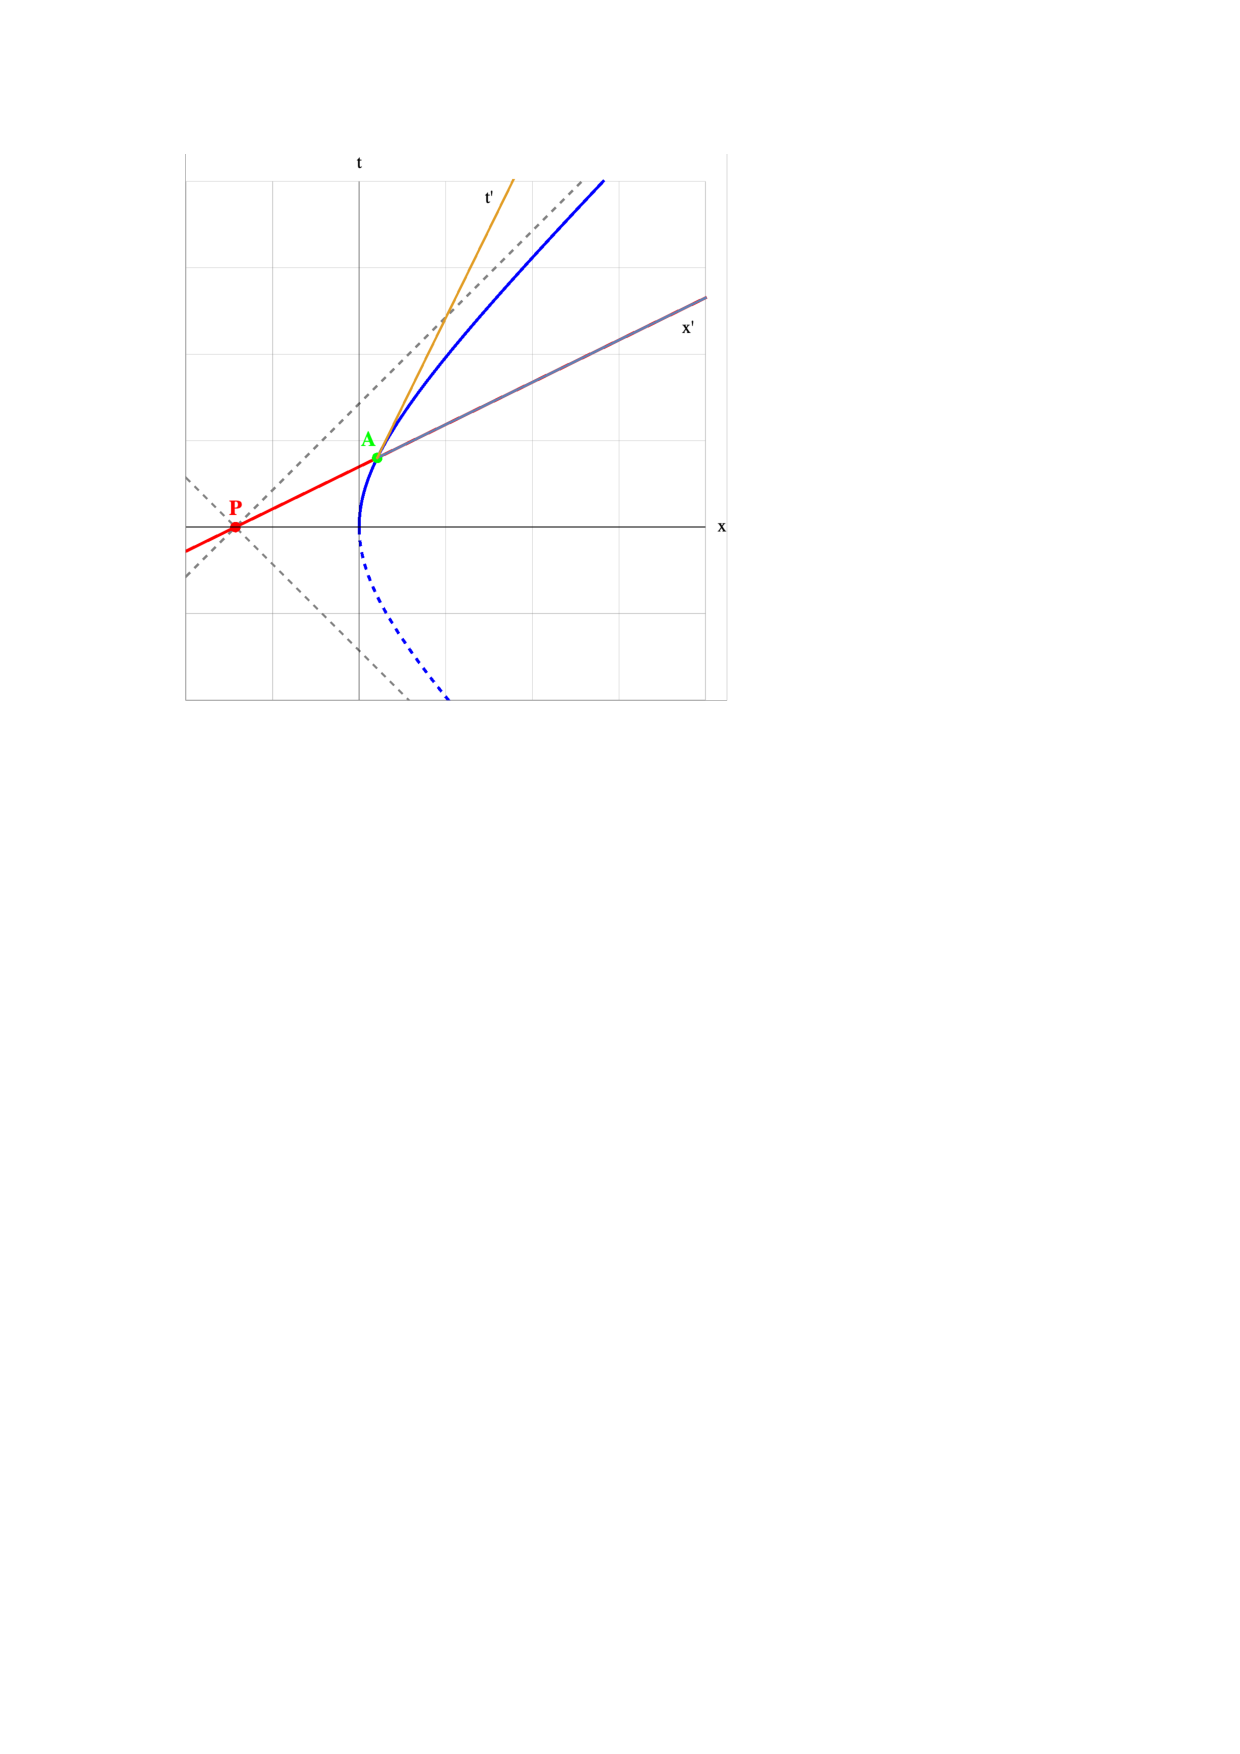
\includegraphics[width=0.5\linewidth]{SpaceTimeA_Ch14.pdf}
    \caption{Spacetime diagram showing point $P$ and an event $A$ on the particle's worldline. In the instantaneous inertial frame at $A$, the $x'$ and $t'$ axes are shown. The particle follows the blue worldline, and its distance to $P$, measured in its instantaneous rest frame, is constant.}
    \label{fig:spacetime1}
\end{figure}

Now consider another point $A$ on the particle's hyperbolic worldline. We write: 
\be
(t_A, x_A) = \left(t_A, \frac{1}{g}\left(\sqrt{1+(gt_A)^2} - 1\right)\right).
\ee
The slope of the line $PA$ is
\be
\frac{t_A- t_P}{x_A - x_P} = \frac{gt_A}{\sqrt{1+(gt_A)^2}} = v_A,
\ee
i.e., the velocity at point $A$ by virtue of the equation for the velocity we derived earlier. This is also the slope of the particle's instantaneous $x'$ axis in the particle's frame $S'$. 

Hence the slope construction works at every event along the worldline. For each such event $A$, the line through $A$ parallel to the instantaneous $x'$ axis is that instantaneous rest frame's line of simultaneity, and it passes through $P$. Thus $P$ is simultaneous with $A$ in \emph{each different} instantaneous rest frame. This does not define one global, observer-independent ``now'': the instantaneous rest frame changes continuously along the accelerated trajectory.

The common null asymptotes of these hyperbolae will become the Rindler horizons below. They provide a useful, limited analogy with horizons near black holes, but they are coordinate-dependent features of flat spacetime, not curvature singularities.

We can also find the distance between point $P$ and point $A$ as measured in $S'$. The Lorentz factor between $S$ and $S'$ is given by:
\be
\gamma = \frac{1}{\sqrt{1-v^2}} = \frac{1}{\sqrt{1-\frac{(gt)^2}{1+(gt)^2}}} = \sqrt{1+(gt)^2}.
\ee
In $S$ the distance between $P$ and $A$ is given by $x_A-x_P = \frac{\sqrt{1+(gt)^2}}{g}$. We use the Lorentz transformations:
\be
\Delta x = \gamma(\Delta x' + v \Delta t'),
\ee
with $\Delta t' = 0$ (this is where we are measuring $\Delta x'$). We thus find:
\be
x_A' - x_P' = \gamma^{-1}(x_A - x_P) = \frac{1}{g} \label{eq:distance}. 
\ee
Hence, the distance between $A$ and $P$ in frame $S'$ is independent of time. So, besides $P$ being simultaneous with any event along the worldline of the trajectory in the particle frame, $P$ is also always the same distance away. So while the particle is accelerating away from point $P$, as observed in the particle's frame, it does not get further away from $P$. This somewhat magical result is the consequence of the fact that, as you accelerate away, and therefore you are moving away from $P$, the distance between you and $P$ keeps contracting. Here we find that these effects exactly cancel.

We can now put a collection of uniformly accelerating particles together to form a uniformly accelerating frame. If all particles accelerate with the same proper acceleration, $g$, the distances between the particles, as measured in the instantaneous inertial frame of the particle, grow larger (see problem 11.26). While this is fine, it is not a frame we would like to work with because of the equivalence principle. Since this states we can not distinguish between a uniformly accelerating frame and a uniform gravitational field, and hence we would like to make sure distances are not affected by moving to this uniformly accelerating frame. Instead, we want to construct a static frame, where distances do not change as measured by an observer comoving with that frame. 

Let us consider two particles, $A$ and $B$. As in the previous example, their worldlines are hyperbolas that share the same null asymptotes through the event $P$ (see the left side of Fig.~\ref{fig:spacetime2}). These null lines form the Rindler horizons; $P$ itself is their intersection, or bifurcation event.

\begin{figure}
    \centering
    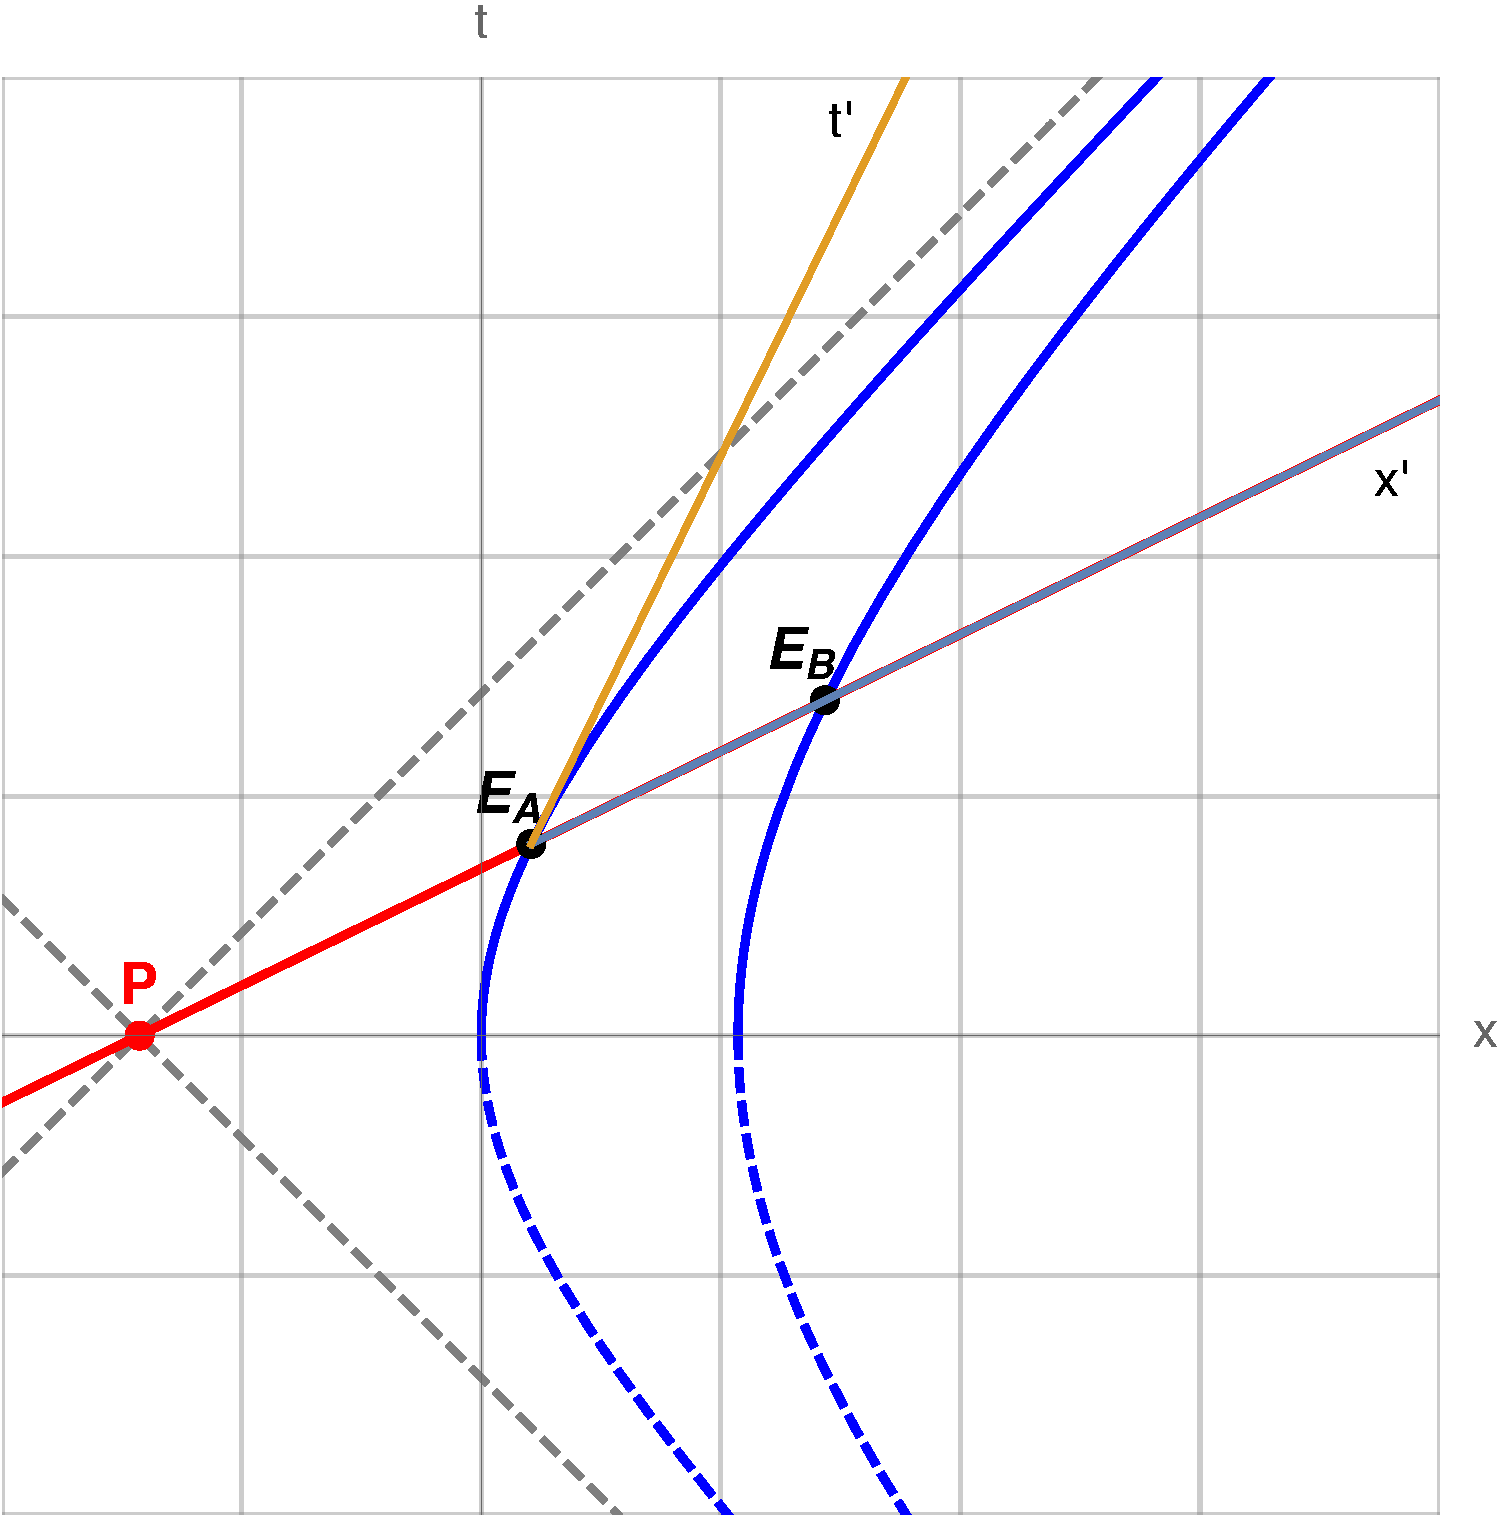
\includegraphics[width=0.45\linewidth]{STDB.pdf}
    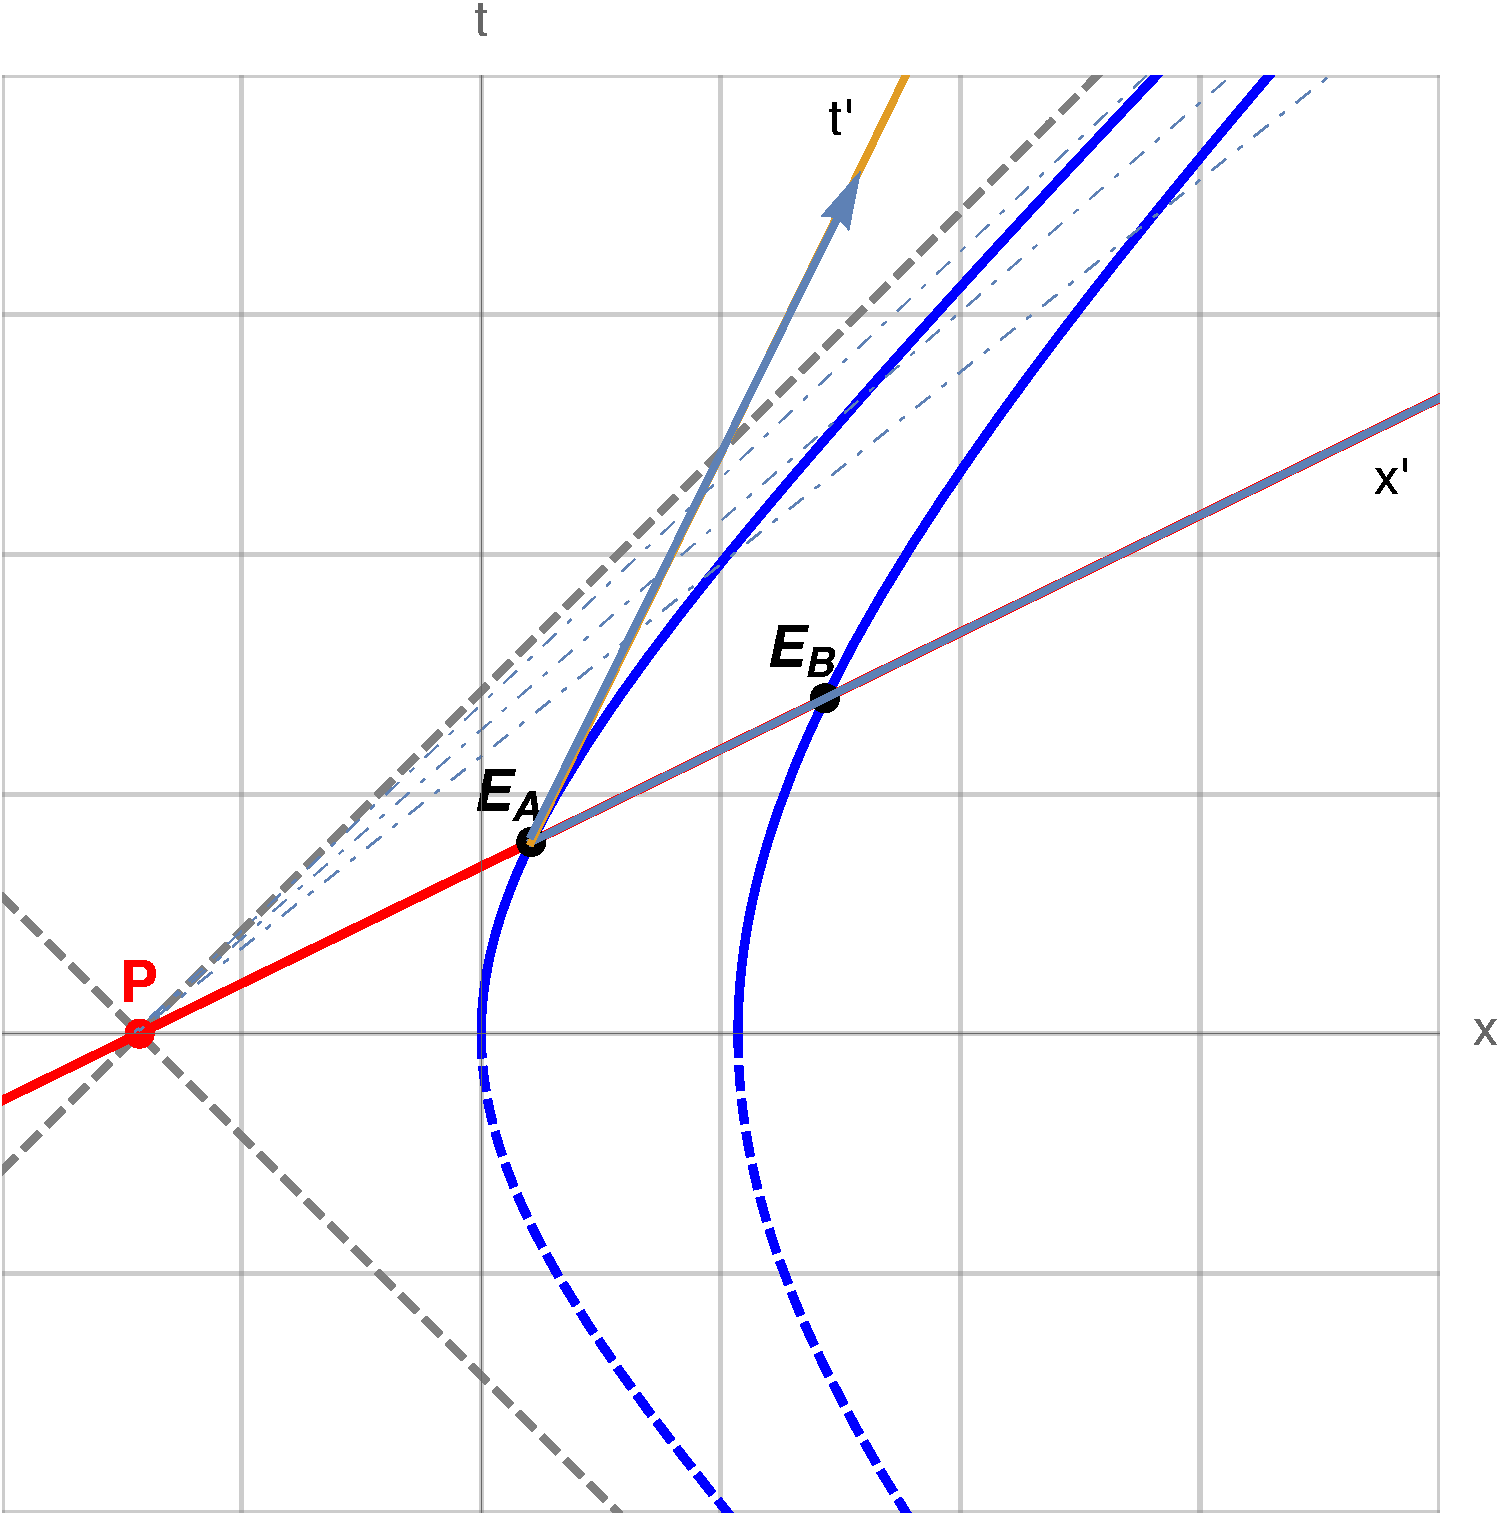
\includegraphics[width=0.45\linewidth]{STDC.pdf}
    \caption{Left: Two particles follow different hyperbolic worldlines with the same null asymptotes through $P$. Initially their proper distances from $P$ are $a$ and $b$, with $g_A=1/a$ and $g_B=1/b$. The events $E_A$, $E_B$, and $P$ lie on a common accelerated-frame simultaneity line. Right: after particle $A$ detaches and follows an inertial straight worldline, it crosses the thick grey dashed Rindler horizon in finite proper time. The thin blue dashed straight lines through $P$ are successive simultaneity lines (the spatial coordinate axes) of $B$'s instantaneous rest frames. They approach the horizon as Rindler time tends to infinity, explaining why the crossing has no finite Rindler time.}
    \label{fig:spacetime2}
\end{figure}


Let the proper distances from $P$ be $a$ for particle $A$ and $b$ for particle $B$. In the $c=1$ units of this section, Eq.~\eqref{eq:distance} gives the required proper accelerations
\be
g_A=\frac{1}{a},\qquad g_B=\frac{1}{b}.
\ee
(With $c$ restored, these read $g_A=c^2/a$ and $g_B=c^2/b$.) Thus, to keep the particles at fixed separations in the accelerated frame, their proper accelerations must be inversely proportional to their distance from $P$.

Now consider two events $E_A$ and $E_B$, such that $P$, $E_A$ and $E_B$ are collinear. The line that passes through these points is, by construction, the $x'$ axis for both particles $A$ and $B$. In addition, $A$ is always a distance $a$ from $P$ and $B$ is always a distance $b$ from $P$. For both particles, length is measured along this $x'$ axis, so the distance between $A$ and $B$ is $b-a$, independent of time. This gives a static accelerated frame, called a Rindler frame. If $\rho$ denotes the instantaneous proper distance to $P$, observers fixed at different Rindler positions require different proper accelerations, $g(\rho)=1/\rho$ (or $c^2/\rho$ with $c$ restored). This is the acceleration needed to remain at rest in these coordinates; it is not a Newtonian gravitational field sourced by matter at $P$.

If this observer detaches from the accelerating frame and subsequently follows an inertial worldline, the accelerated-frame description resembles free fall. The observer crosses the null Rindler horizon in finite proper time, because the straight inertial worldline intersects the common asymptote of the hyperbolic worldlines (see the right side of Fig.~\ref{fig:spacetime2}). The observer does not pass through the event $P$ in general.

Observers who continue accelerating along the hyperbolic worldlines remain at fixed Rindler positions. Using their accelerated coordinate system, the detached observer approaches the horizon as Rindler time tends to infinity. The detached observer nevertheless crosses the horizon in finite proper time; nothing singular happens there locally. The horizon is a boundary of the accelerated coordinate system, while the underlying Minkowski spacetime is regular there.

The thin blue dashed straight lines in the right-hand panel of Fig.~\ref{fig:spacetime2} show how this works geometrically. At each event on $B$'s hyperbolic worldline, the spatial axis of its instantaneous rest frame passes through $P$ and selects the events simultaneous with that event on $B$. As $B$ continues accelerating, these simultaneity lines tilt toward the future Rindler horizon. Let $H$ denote the event where the detached particle crosses that horizon. For $H$ to lie on one of these simultaneity lines, the line through $P$ would have to coincide with the horizon itself. This alignment is approached only as Rindler time tends to infinity; no instantaneous rest frame at a finite time on $B$ assigns $H$ to its current simultaneity line. This is a statement about assigning coordinate time, not about receiving light signals, and it does not prevent the detached particle from reaching $H$ in finite proper time.

This provides a useful local analogy with a black hole. A freely falling observer crosses a black-hole horizon in finite proper time, while Schwarzschild coordinates assign the crossing an infinite coordinate time; signals received far away become increasingly delayed and redshifted. The equivalence principle motivates the local connection between acceleration and gravity, but the global structure of a black-hole spacetime requires general relativity and is not derived from the Rindler analogy alone.





\ifshowboardquestion
\section*{Board Question}
\begin{tcolorbox}[colback=blue!5!white]
An observer undergoes constant proper acceleration $a$ in flat spacetime.
\begin{enumerate}
    \item Sketch the observer's worldline on a spacetime diagram.
    \boardanswer{The worldline is a hyperbola in the future wedge, e.g. $x^2-c^2t^2=c^4/a^2$ for suitable initial conditions.}
    \item Explain why the worldline approaches, but never crosses, a lightlike asymptote.
    \boardanswer{As inertial-frame time grows, the coordinate velocity approaches $c$, so the worldline approaches a lightlike line without crossing it.}
    \item Describe what this means for the observer's coordinate acceleration in an inertial frame.
    \boardanswer{The proper acceleration stays constant, but the coordinate acceleration decreases and tends to zero as the speed approaches $c$.}
    \item Use the equivalence principle to relate this situation locally to an observer at rest in a uniform gravitational field.
    \boardanswer{Locally, a uniformly accelerated observer in flat spacetime is equivalent to an observer at rest in a gravitational field of strength $a$.}
\end{enumerate}
\end{tcolorbox}
\fi

\end{document}
